\chapter{2018年「大学物理2」\titlelogo{https://sci.hdu.edu.cn}{HDU}期中试题}
\date{2018年11月11日}{大学物理教学团队}{A0715012}
{未央物理讲师 \href{https://qm.qq.com/q/UPbGudx8cK}{\textbf{Axia}}}
{\qrcode{https://h5.qun.qq.com/s/WRps3LNC8K}}{\href{https://h5.qun.qq.com/s/WRps3LNC8K}{HDU 物理营}}
{\qrcode{http://weixin.qq.com/r/mhKYgFTEMQlOrRDj90eI}}{\href{http://weixin.qq.com/r/mhKYgFTEMQlOrRDj90eI}{未央学社公众号}}

\section{选择题（每题3分，共27分）}
\begin{choice}{C}[简谐振动]
    一沿$x$轴做简谐振动的弹簧振子，振幅为$A$，周期为$T$，振动方程用余弦函数表示，如果该振子的初相为$\frac{3}{4}\pi$，则$t=0$时刻，质点的位置在
    \begin{tasks}(2)
        \task 过$x=+\frac{\sqrt{2}}{2}A$处，向负方向运动
        \task 过$x=-\frac{\sqrt{2}}{2}A$处，向正方向运动
        \task 过$x=-\frac{\sqrt{2}}{2}A$处，向负方向运动
        \task 过$x=+\frac{\sqrt{2}}{2}A$处，向正方向运动
    \end{tasks}
\end{choice}

\begin{choice}{B}[简谐振动]
    一质点沿$x$轴做简谐振动，振动方程为$x=0.08\cos{\ab(\pi t+\frac{1}{3}\pi)}$ (\textbf{SI}).从$t=0$时刻起，到质点位置在$x=-0.04\mathrm{m}$处，且向$x$轴正方向运动的最短时间间隔为
    \begin{tasks}(4)
        \task $\frac{1}{2}\mathrm{s}$
        \task $1\mathrm{s}$
        \task $2\mathrm{s}$
        \task $3\mathrm{s}$
    \end{tasks}
\end{choice}
\begin{solution}*
    此时质点的相位为$\varphi=\frac{4}{3}\pi$，则相位变化$\Delta\varphi=\pi$，时间间隔$\Delta t=\frac{\Delta\varphi}{\omega}=1\mathrm{s}$.\sokka{B}
\end{solution}

\begin{choice}{D}[驻波]
    沿着相反方向传播的两列相干波，其表达式为
    \[y_1=A\cos{2\pi\ab(\nu t-\frac{x}{\lambda})},\ y_2=A\cos{2\pi\ab(\nu t+\frac{x}{\lambda})}\]

    叠加后形成的驻波中，波腹的位置坐标为（其中$k=0,1,2,3,\cdots$）
    \begin{tasks}(4)
        \task $x=\pm k\lambda$
        \task $x=\pm(2k+1)\lambda/4$
        \task $x=\pm(2k+1)\lambda/2$
        \task $x=\pm k\lambda/2$
    \end{tasks}
\end{choice}
\begin{solution}*
    形成的驻波表达式为，$y=y_1+y_2=2A\cos(2\pi\nu t)\cos(2\pi x/\lambda)$，故波腹位置坐标为$x=\pm k\lambda/2$.
\end{solution}

\begin{paracol}{2}
\begin{choice}{B}[波的能量]
    图示为一平面简谐机械波在$t$时刻的波形曲线.若此时$A$点处媒质质元的振动动能在增大，则
    \begin{tasks}(2)
        \task $A$点处质元的弹性势能在减小
        \task 波沿$x$轴负方向传播
        \task $B$点处质元的振动动能在减小
        \task 各点能量密度都不随时间变化
    \end{tasks}
\end{choice}
\switchcolumn\centering
\vfill
    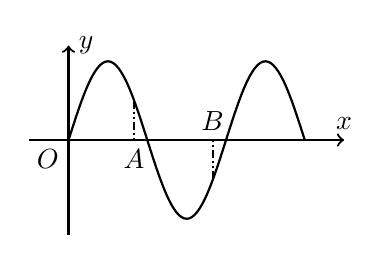
\begin{tikzpicture}
        \draw [thick,->] (-0.5,0)--(3.5,0) node [anchor=south] {$x$};
        \draw [thick,->] (0,-1.2)--(0,1.2) node [anchor=west] at (0,1.2) {$y$};
        \draw [thick] (0,0) sin (0.5,1) cos (1,0) sin (1.5,-1) cos (2,0) sin (2.5,1) cos (3,0);
        \node [anchor=north east] at (0,0) {$O$};
        \draw [thick,densely dash dot dot] (0.83,0.5)--(0.83,0);
        \draw [thick,densely dash dot dot] (1.83,-0.5)--(1.83,0);
        \node [anchor=north] at (0.83,0) {$A$} node [anchor=south] at (1.83,0) {$B$};
    \end{tikzpicture}
\vfill
\end{paracol}
\begin{solution}
    \begin{itemize}
        \item $A$点的振动动能在增大，所以$A$点在靠近平衡位置，波沿$x$轴负方向传播，B项正确
        \item 波沿$x$轴负方向传播，由图可知$B$点在靠近平衡位置，其振动动能在增大，C项错误
        \item 根据机械波的特性：动能和势能同时增大或减小，能量密度随时间变化，A、D项错误
    \end{itemize}
\end{solution}

\begin{choice}{B}[驻波]
    在驻波中，两个相邻波节间各质点的振动
    \begin{tasks}(4)
        \task 振幅相同，相位相同
        \task 振幅不同，相位相同
        \task 振幅相同，相位不同
        \task 振幅不同，相位不同
    \end{tasks}    
\end{choice}
\begin{solution}*
    根据驻波波形的特点「波形并不向前推进，而是在介质中来回振荡」.\sokka{B}
\end{solution}

\begin{choice}{A}[多普勒效应]
    一机车汽笛频率为$550\mathrm{Hz}$，机车以$30\mathrm{m/s}$的速度驶近静止的观察者，观察者听到声音的频率是（空气中声速$330\mathrm{m/s}$）
    \begin{tasks}(4)
        \task $605\mathrm{Hz}$
        \task $600\mathrm{Hz}$
        \task $504\mathrm{Hz}$
        \task $500\mathrm{Hz}$
    \end{tasks}
\end{choice}
\begin{solution}
    已知多普勒效应观察者（Observer）和发射源（Source）的的频率关系为
    \[\nu=\frac{u\pm v_o}{u\mp v_s}\nu_0\]

    $v_o$为观察者速度，接近为$+$，远离为$-$；$v_s$为发射源速度，接近为$-$，远离为$+$.观察者静止，其所听频率为
    \[\nu=\frac{330}{330-30}\times 550\mathrm{Hz}\approx 605\mathrm{Hz}\]

    \sokka{C}
\end{solution}

\begin{paracol}{2}
    \begin{choice}{A}[双缝干涉]
        如图所示，用波长$\lambda=600\mathrm{nm}$的单色光做杨氏双缝实验，在光$P$处产生第5级明纹极大，现将折射率$n=1.5$的薄透明玻璃片盖在其中一条缝上，此时$P$处变成第一级明纹极大的位置，则此玻璃片厚度为
        \begin{tasks}(4)
            \task $4.8\times 10^{-4}\mathrm{cm}$
            \task $6.0\times 10^{-4}\mathrm{cm}$
            \task $7.2\times 10^{-4}\mathrm{cm}$
            \task $8.4\times 10^{-4}\mathrm{cm}$
        \end{tasks}
    \end{choice}
    \switchcolumn\centering
    \vfill
    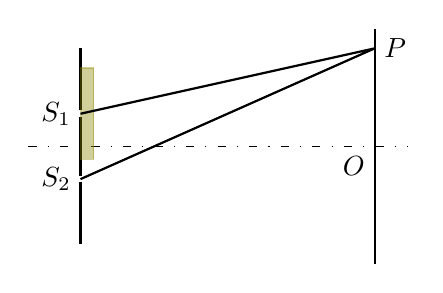
\begin{tikzpicture}[scale=0.83]
        \draw [thick] (0,1.5)--(0,0.55);
        \draw [thick] (0,0.45)--(0,-0.45);
        \draw [thick] (0,-0.55)--(0,-1.5);
        \draw [loosely dash dot] (-0.8,0)--(5,0);
        \draw [thick] (4.5,1.8)--(4.5,-1.8);
        \filldraw [olive,opacity=0.4] (0,1.2) rectangle (0.2,-0.2);
        \draw [thick] (0,0.5)--(4.5,1.5)--(0,-0.5);
        \node [anchor=east] at (0,0.5) {$S_1$} node [anchor=east] at (0,-0.5) {$S_2$};
        \node [anchor=west] at (4.5,1.5) {$P$};
        \node [anchor=north east] at (4.5,0) {$O$};
    \end{tikzpicture}
    \vfill
\end{paracol}
\begin{solution}*
    遮住后光程差变化$5\lambda-\lambda=2400\mathrm{nm}=\ab(n-1)e$，得玻璃片厚度$e=4.8\times 10^{-4}\mathrm{cm}$.\sokka{A}
\end{solution}

\begin{choice}{D}[劈尖干涉]
    两块平玻璃构成空气劈尖，左边为棱边，用单色平行光垂直入射，若上面的平玻璃慢慢地向上平移，则干涉条纹
    \begin{tasks}(2)
        \task 向棱边方向平移，条纹间隔变小
        \task 向远离棱的方向平移，条纹间隔不变
        \task 向远离棱的方向平移，条纹间隔变大
        \task 向棱边方向平移，条纹间隔不变
    \end{tasks}
\end{choice}
\begin{solution}*
    平移过程中空气劈形膜的顶角不变，所以条纹间隔不变；平移过程中每处的光程差增大，所以对应的条纹级数增大，表现为向棱边方向平移.\sokka{D}
\end{solution}

\begin{choice}{C}[弗琅禾费衍射]
    在单缝夫琅和费衍射实验中，波长为$\lambda$的单色光垂直入射在宽度为$a=6\lambda$的单缝上，对应于衍射角为$30^{\circ}$的方向，单缝处波阵面可分成的半波带数目为
    \begin{tasks}(4)
        \task 2个
        \task 4个
        \task 6个
        \task 8个
    \end{tasks}
\end{choice}
\begin{solution}*
    由衍射公式$a\sin{\theta}=k\lambda$得$k=3$，可分成的半波带数目为$2k=6$.\sokka{C}
\end{solution}

\section{填空题（共25分）}
\begin{paracol}{2}
    
\begin{problem}[平面简谐波的物理量][4]
    一平面简谐波沿$x$轴正方向传播，波速$u=120\mathrm{m/s}$，$t=0$时刻的波形曲线如图所示，则简谐波的波长\ans{$0.8\mathrm{m}$}， 频率\ans{$150\mathrm{Hz}$}.
\end{problem}
\begin{solution}*
    由图易知波长$\lambda=0.8\mathrm{m}$；简谐波的频率$f=\frac{u}{\lambda}=150\mathrm{Hz}$.
\end{solution}
\switchcolumn\centering
\vfill
\begin{tikzpicture}[decoration={markings,
    mark=between positions 0.0625 and 1 step 6mm
    with {\draw [-,darkgray] (0,-0.1) -- (0,0.1);}},scale=1,xscale=1.2]
    \draw [thick,->,postaction=decorate] (-0.2,0)--(3,0) node [anchor=south] {$x/\mathrm{m}$};
    \draw [thick,->] (0,-1.2)--(0,1.5) node [anchor=south] {$y/\mathrm{m}$};
    \node [anchor=north east] at (0,0) {$O$};
    \draw [thick] (0,1) cos (0.5,0) sin (1,-1) cos (1.5,0) sin (2,1) cos (2.5,0);
    \draw [very thick,->] (0.6,1.2)--(1.8,1.2) node [anchor=south,midway] {$u$};
    \node [anchor=north] at (0.5,0) {$0.2$} node [anchor=north] at (1.0,0) {$0.4$} node [anchor=north] at (1.5,0) {$0.6$} node [anchor=north] at (2.0,0) {$0.8$} node [anchor=north] at (2.5,0) {$1.0$} node [anchor=east] at (0,1) {$0.2$};
\end{tikzpicture}
\vfill
\end{paracol}

\begin{paracol}{2}
    \begin{problem}[光程和光程差][3]
        如图所示，两相干波源$S_1$和$S_2$相距$\frac{\lambda}{4}$，$S_1$的相位比$S_2$的相位超前$\frac{\pi}{3}$.在$S_1S_2$的连线上两者外侧$P$点两波引起的简谐振动的相位差是\ans{$\frac{5\pi}{6}$}.
    \end{problem}
\switchcolumn\centering
\vfill
\begin{tikzpicture}
    \draw [very thick,1号色] (-2.4,0)--(2.4,0);
    \length{(0,-0.5)}{(2,-0.5)}{$\frac{1}{4}\lambda$}{(0.5,0)}
    \shade[ball color=red!40] (-2,0) circle (0.05);
    \shade[ball color=red!40] (0,0) circle (0.05);
    \shade[ball color=red!40] (2,0) circle (0.05);
    \node [anchor=south] at (-2,0) {P};
    \node [anchor=south] at (0,0) {$S_1$} node [anchor=south] at (2,0) {$S_2$};
\end{tikzpicture}
\vfill
\end{paracol}
\begin{solution}*
    因传播过程而造成的相位差为$\frac{2\pi\delta}{\lambda}=\frac{2\pi\cdot\lambda/4}{\lambda}=\frac{\pi}{2}$，又因为$S_1$的相位比$S_2$的相位超前$\frac{\pi}{3}$，所以$P$点处两波引起的相位差为$\frac{5\pi}6$.
\end{solution}

\begin{problem}[简谐振动][3]
    用$40\mathrm{N}$的力拉一轻弹簧，可使其伸长$20\mathrm{cm}$.此弹簧下应挂\ans{$0.5$}$\mathrm{kg}$的物体，才能使其做简谐振动的周期为$T=0.1\pi$.
\end{problem}
\begin{solution}*
    弹簧劲度系数$k=40\mathrm{N}/0.2\mathrm{m}=200\mathrm{N/m}$；由振子振动周期$T=2\pi\sqrt{m/k}$得$m=kT^2/4\pi^2=0.5\mathrm{kg}$.
\end{solution}

\begin{problem}[光的相干条件][3]
    在双缝干涉实验中，用白光照射时，明纹会出现彩色条纹，明纹外侧呈\ans{红}颜色；如果用纯绿色滤光片和纯蓝色滤光片分别盖住两缝，则\ans{不能}产生干涉条纹（填能或不能）.
\end{problem}
\begin{solution}*
    波长越大，明纹张角越大，所以外侧呈红色；根据干涉条件「频率相等」，此时不能产生干涉条纹.
\end{solution}

\begin{problem}[相干光的叠加后的光强分布][3]
    光强均为$I_0$的两束相干光发生干涉时，在相遇区域内可能出现的最大光强是\ans{$4I_0$}，可能出现的最小光强是\ans{$0$}.
\end{problem}
\begin{solution}*
    两种情况分别对应「干涉相长」与「干涉相消」，即$I=I_1+I_2\pm 2\sqrt{I_1I_2}$，对应光强分别为$4I_0$与$0$.
\end{solution}

\begin{problem}[增透膜][3]
    在照相机镜头的玻璃片上均匀镀有一层折射率为$n$的介质薄膜（$n$大于玻璃的折射率），以增强某一波长$\lambda$的透射光能量.假设光线垂直入射，则介质膜的最小厚度应为\ans{$\frac{\lambda}{2n}$}.
\end{problem}
\begin{solution}
    \begin{itemize}
        \item \textbf{当光从光密介质射向光疏介质时，反射光没有半波损失}.所以两个表面反射光光程差为$\delta=2ne+\frac\lambda2$.
        \item 使反射光干涉相消，即$2ne+\frac\lambda2=\frac{2k+1}{2}\lambda$. 解得$k=1$时，$e_{\min}=\frac{\lambda}{2n}$.
    \end{itemize}
\end{solution}

\begin{problem}[牛顿环][3]
    波长$\lambda=600\mathrm{nm}$的单色光垂直照射到牛顿环的装置上，第三级明纹与第七级明纹所对应的空气膜厚度之差为\ans{$1200$}$\mathrm{nm}$.
\end{problem}
\begin{solution}
    由明环半径公式$r_k=\sqrt{\frac{2k-1}{2}\lambda R}$得第三级明纹与第七级明纹所对应的空气膜厚度之差为
    \[\Delta d=\sqrt{R^2-r_3^2}-\sqrt{R^2-r_7^2}\xlongequal[\lambda\ll R]{\sqrt{1-\frac{\lambda}{R}}\sim1-\frac{\lambda}{2r}}R\ab(1-\frac{5\lambda}{4R})-R\ab(1-\frac{13\lambda}{4R})=2\lambda=600\mathrm{nm}\]
\end{solution}

\begin{problem}[弗琅禾费衍射][3]
    测量未知单缝宽度$a$的一种方法是：用已知波长$\lambda$的平行光垂直入射在单缝上，在距单缝的距离为$f$处测出衍射花样的中央亮纹宽度为$L$（实验上保证$f\approx 10^3a$），则由单缝衍射的原理可标出$a$与$\lambda$，$f$，$L$的关系为$a=$\ans{$\frac{2\lambda f}{L}$}.
\end{problem}
\begin{solution}*
    由衍射公式$a\sin{\theta}=\lambda$得中央明纹张角$2\theta\approx\frac{2\lambda}{a}$，所以中央明纹宽度$L=\frac{2\lambda f}{a}$，即$a=\frac{2\lambda f}{L}$.
\end{solution}

\section{计算题（共48分）}
\begin{problem}[简谐振动][10]
    一质点按如下规律沿$x$轴做简谐振动
    \[x=0.2\cos{\ab(4\pi t+\frac{1}{3}\pi)}\ \mathrm{(SI)}\]
    
    求此振动的周期、振幅、初相、速度最大值和加速度最大值.
\end{problem}
\begin{solution}
    \begin{multicols}{2}
    \begin{itemize}
        \item 周期：$T=2\pi/\omega=0.5\mathrm{s}$\point{2}
        \item 振幅：$A=0.2\mathrm{m}$\point{2}
        \item 初相：$\varphi_0=\frac{1}{3}\pi$\point{2}
        \item 速度最大值：$v_{\max}=\omega A=0.8\pi\mathrm{m/s}$\point{2}
        \item 加速度最大值：$a_{\max}=\omega^2 A=3.2\pi^2\mathrm{m/s}^2$\point{2}
    \end{itemize}
\end{multicols}
\end{solution}

\begin{problem}[简谐振动，平面简谐波的波函数][8]
    某质点做简谐振动，周期为$3\mathrm{s}$，振幅为$0.5\mathrm{m}$，$t=0$时刻，质点恰好处在平衡位置并向正方向运动，求
    \begin{enumerate}
        \item 该质点的振动方程.
        \item 此振动以速度$u=5\mathrm{m/s}$沿$x$轴正方向传播时，形成的一维简谐波的波动方程（以平衡位置为坐标原点）.
        \item 该波的波长.
    \end{enumerate}
\end{problem}
\begin{solution}
    \begin{enumerate}
        \item 由题意得，质点的角频率$\omega=\frac{2\pi}{T}=\frac{2\pi}{3}\mathrm{s}^{-1}$，质点的初相$\varphi=-\frac{\pi}{2}$.故质点的振动方程为\point{1}
        \[y_0=0.5\cos{\ab(\frac{2\pi}{3}t-\frac{\pi}{2})}\eqno\point{2}\]
        \item 波动表达式
        \[y=A\cos{\ab[\omega\ab(t-\frac{x}{u})+\varphi]}=0.5\cos{\ab[\frac{2\pi}{3}\ab(t-\frac{x}{5})-\frac{\pi}{2}]}\eqno\point{3}\]
        \item 波长$\lambda=uT=15\mathrm{m}$.\point{2}
    \end{enumerate}
\end{solution}

\begin{problem}[牛顿环][10]
    用波长$\lambda=780\mathrm{nm}$ 的单色光做牛顿环实验，测得第$k$个暗环半径$r_k=4\mathrm{mm}$，第$k+6$个暗环半径$r_{k+6}=7\mathrm{mm}$，求平凸透镜的凸面的曲率半径$R$.
\end{problem}
\begin{solution}*
    根据暗环半径公式$r_k=\sqrt{k\lambda R},\ r_{k+6}=\sqrt{\ab(k+6)\lambda R}$得$R=\ab(r_{k+6}^2-r_k^2)/6\lambda=7.05\mathrm{m}$.
\end{solution}

\begin{paracol}{2}
    \begin{problem}[双缝干涉][10]
        双缝干涉实验装置如图所示, 双缝与屏之间的距离$D=150\mathrm{cm}$, 两缝之间的距离$d=0.50\mathrm{mm}$, 用波长$\lambda=600\mathrm{nm}$的单色光垂直照射双缝.
        \begin{enumerate}
            \item 求原点$O$（零级明条纹所在处）上方第3级明条纹的坐标
            \item 如果用厚度$e=0.02\mathrm{mm}$，折射率$n=1.67$的透明薄膜覆盖在图中的$S_1$缝后面，求上述第3级明条纹的坐标$x^{\prime}$.
        \end{enumerate}
    \end{problem}
    \switchcolumn\centering
    \vfill
    \begin{tikzpicture}[scale=0.48]
        \draw [dash dot] (-0.2,0)--(6.2,0);
        \draw (0,1.5)--(0,3);
        \draw (0,-1)--(0,1);
        \draw (0,-1.5)--(0,-3);
        \draw [2号色,thick] (0,1.25)--(6,2.25);
        \draw [2号色,thick] (0,-1.25)--(6,2.25);
        \draw (6,3)--(6,-3);
        \draw [<->] (0,-2.5)--(6,-2.5) node [anchor=south,midway] {$D$};
        \node [anchor=south west] at (0,1.25) {$S_1$} node [anchor=north west] at (0,-1.25) {$S_2$};
        \node [anchor=east] at (0,0) {$d$};
        \draw[->] (-1.25,1.25)--(-0.2,1.25);
        \draw[->] (-1.25,-1.25)--(-0.2,-1.25);
    \end{tikzpicture}
    \vfill
\end{paracol}
\begin{solution}
    \begin{enumerate}
        \item $x_3=\frac{3\lambda D}{d}=5.4\mathrm{mm}$.\point{4}
        \item 根据明纹条件，此时的光程差为
        \[\delta=r_2-r_1-\ab(n-1)e=\frac{x_3^{\prime}d}{D}-\ab(n-1)e=k\lambda\eqno\point{4}\]

        得$x_3^{\prime}=\ab[k\lambda+\ab(n-1)e]\frac{D}{d}=45.6\mathrm{mm}$.\point{2}
    \end{enumerate}
\end{solution}

\begin{problem}[弗琅禾费衍射][10]
    波长为$760\mathrm{nm}$的平行光垂直地入射于一宽为$0.5\mathrm{mm}$的狭缝，若在缝的后面有一焦距为$2\mathrm{m}$的薄透镜，使光线会聚于一屏幕上，试求
\begin{enumerate}
    \item 中央明纹宽度
    \item 第一级明纹的位置，两侧第二级暗纹之间的距离（$1\mathrm{nm}=10^{-9}\mathrm{m}$）.
\end{enumerate}
\end{problem}
\begin{solution}
    \begin{enumerate}
        \item 中央明条纹宽度$\Delta x_0=\frac{2\lambda f}{a}=6.08\mathrm{mm}$.\point{3}
        \item 第一级明纹位置$a\sin{\varphi_1}=\pm\ab(2k+1)\frac{\lambda}{2}=\pm\frac32\lambda$，$x_1=f\sin{\varphi_1}=\frac{3\lambda f}{2a}=\pm 4.56\mathrm{mm}$.\point{3}
        
        第二级暗纹位置$a\sin{\varphi_2}=\pm k\lambda=\pm 2\lambda$，$\Delta x_2=\abs{2\cdot f\sin\varphi_2}=\frac{4\lambda f}{a}=12.16\mathrm{mm}$.\point{3}
    \end{enumerate}
\end{solution}